\chapter{幂指对函数}
\begin{introduction}
    \item 幂函数
    \item 指数函数
    \item 对数函数
    \item 双钩函数
\end{introduction}

\section{幂函数}

\subsection{幂函数的定义}

\begin{definition}[幂函数]
    形如$f(x)=x^k$（其中$k\in \mathbb{Q}$为常数）的函数称为幂函数。
\end{definition}

\begin{example}
    下列函数中是幂函数的是 （\qquad）
    \begin{tasks}(4)
        \task $y=\sqrt{x}$
        \task $y=x^3$
        \task $y=3 x$
        \task $y=x^{-1}$
    \end{tasks}
\end{example}

\v{2em}

\begin{example}
    下列函数中，为幂函数的是 （\qquad）
    \begin{tasks}(4)
        \task $f(x)=x^3$
        \task $f(x)=2 x^2$
        \task $f(x)=x^{-1}$
        \task $f(x)=2^x$
    \end{tasks}
\end{example}

\v{2em}

\begin{note}[幂运算]
    从小学到初中我们依次学会了：
    \begin{enumerate}
        \item     正整数幂：$x^2 = x\times x$
        \item     负整数幂：$x^{-n} = \frac{1}{x^n}$
        \item     分数幂：$x^{\frac{1}{n}} = \sqrt[n]{x}$
    \end{enumerate}
    于是我们可以算出所有的有理数幂：$$x^{\frac{p}{q}} = \sqrt[q]{x^p}$$
\end{note}

\begin{warning}
    幂函数前的系数一定是 $1$.
\end{warning}

\begin{example}
    幂函数 $f(x)=\left(m^2-m-1\right) x^m$ 在 $(0,+\infty)$ 上单调递增，求 $m$ 的值。
\end{example}

\v{4em}

\subsection{幂函数的图像}

幂函数的性质取决于$k$的取值。
$k=0$ 和 $k$ 为正整数：
\begin{figure}[H]
    \centering
    \begin{minipage}[b]{0.45\textwidth}
        \centering
        \begin{tikzpicture}[scale=0.6]
            \draw[<->](3,0)--(0,0)--(0,3);
            \draw(0,-2)--(0,0)--(-3,0);
            \draw[blue,domain=-1.8:1.8] plot(\x,1);
        \end{tikzpicture}
        \caption{$y=1$ ($k=0$)}
    \end{minipage}
    \hfill
    \begin{minipage}[b]{0.45\textwidth}
        \centering
        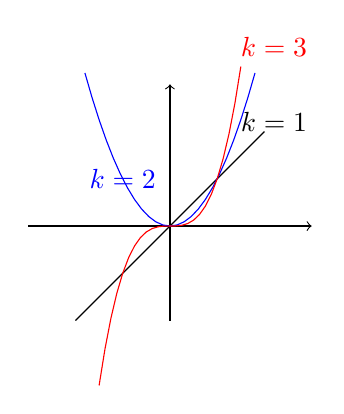
\begin{tikzpicture}[scale=0.6]
            \draw[<->](3,0)--(0,0)--(0,3);
            \draw(0,-2)--(0,0)--(-3,0);
            \draw[black,domain=-2:2] plot(\x,\x) node at (2.2,2.2) {$k=1$};
            \draw[blue,domain=-1.8:1.8] plot(\x,\x*\x) node at (-1,1) {$k=2$};
            \draw[red,domain=-1.5:1.5] plot(\x,\x^3) node at (2.2,3.8) {$k=3$};
        \end{tikzpicture}
        \caption{$k$ 为正整数}
    \end{minipage}

    \vspace{1em}

    \begin{minipage}[b]{0.45\textwidth}
        \centering
        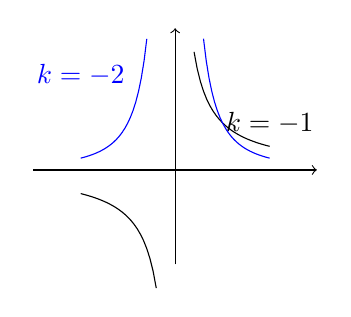
\begin{tikzpicture}[scale=0.6]
            \draw[<->](3,0)--(0,0)--(0,3);
            \draw(0,-2)--(0,0)--(-3,0);
            \draw[black,domain=-2:-0.4] plot(\x,1/\x) node at (2,1) {$k=-1$};
            \draw[black,domain=0.4:2] plot(\x,1/\x);
            \draw[blue,domain=-2:-0.6] plot(\x,{1/(\x)^2}) node at (-2,2) {$k=-2$};
            \draw[blue,domain=0.6:2] plot(\x,{1/(\x)^2});
        \end{tikzpicture}
        \caption{$k$ 为负整数}
    \end{minipage}
    \hfill
    \begin{minipage}[b]{0.45\textwidth}
        \centering
        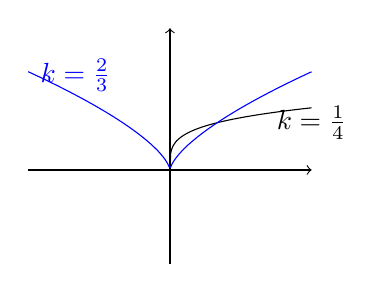
\begin{tikzpicture}[scale=0.6]
            \draw[<->](3,0)--(0,0)--(0,3);
            \draw(0,-2)--(0,0)--(-3,0);
            \draw[black,domain=0:3,samples=200] plot(\x,{\x^0.25}) node at (3,1) {$k=\frac{1}{4}$};
            \draw[blue,domain=-3:3,samples=200] plot(\x,{((\x)^2)^(1/3))}) node at (-2,2) {$k=\frac{2}{3}$};
        \end{tikzpicture}
        \caption{$k$ 为分数}
    \end{minipage}
    \caption{幂函数 $y=x^k$ 的图像}
\end{figure}

\begin{tips}
    分数的情况较为复杂，如果分母是偶数那么根据分数幂的定义，自变量不能取负值。
\end{tips}

\section{指数函数}

\subsection{指数函数的定义}

\begin{definition}[指数函数]
    形如$f(x)=a^x$（其中$a>0$为常数）的函数称为指数函数。
\end{definition}

\subsection{指数函数的图像}

指数函数的图像较为简单，不考虑$a=1$这种非平凡情况。

当$a>1$时，函数单调增：
\begin{figure}[H]
    \centering
    \begin{minipage}[b]{0.45\textwidth}
        \centering
        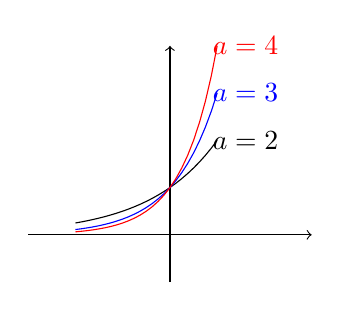
\begin{tikzpicture}[scale=0.6]
            \draw[<->](3,0)--(0,0)--(0,4);
            \draw(0,-1)--(0,0)--(-3,0);
            \draw[black,domain=-2:1] plot(\x,{2^(\x)}) node at (1.6,2) {$a=2$};
            \draw[blue,domain=-2:1] plot(\x,{3^(\x)}) node at (1.6,3) {$a=3$};
            \draw[red,domain=-2:1] plot(\x,{4^(\x)}) node at (1.6,4) {$a=4$};
        \end{tikzpicture}
        \caption{$a>1$，函数单调增}
    \end{minipage}
    \hfill
    \begin{minipage}[b]{0.45\textwidth}
        \centering
        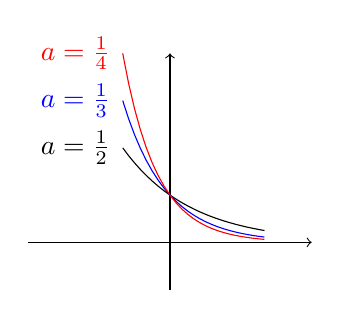
\begin{tikzpicture}[scale=0.6]
            \draw[<->](3,0)--(0,0)--(0,4);
            \draw(0,-1)--(0,0)--(-3,0);
            \draw[black,domain=-1:2] plot(\x,{(1/2)^(\x)}) node at (-2,2) {$a=\frac{1}{2}$};
            \draw[blue,domain=-1:2] plot(\x,{(1/3)^(\x)}) node at (-2,3) {$a=\frac{1}{3}$};
            \draw[red,domain=-1:2] plot(\x,{(1/4)^(\x)}) node at (-2,4) {$a=\frac{1}{4}$};
        \end{tikzpicture}
        \caption{$a<1$，函数单调减}
    \end{minipage}
    \caption{指数函数 $y=a^x$ 的图像}
\end{figure}

\begin{theorem}[指数函数运算性质]
    $(a>0, b>0, r, s \in \mathbf{R})$
    \begin{enumerate}
        \item $a^r a^s=a^{r+s}, \frac{a^r}{a^s}=a^{r-s}$ ；
        \item $\left(a^s\right)^r=a^{r s}=\left(a^r\right)^s(a>0)$ ；
        \item $(a b)^r=a^r b^r$ ；
        \item $a^{\frac{m}{n}}=(\sqrt[n]{a})^m=\sqrt[n]{a^m}(a>0, n, m \in \mathbf{N_+})$
        \item 当 $n$ 为奇数时，$\sqrt[n]{a^n}=a$ ；当 $n$ 为偶数时，$\sqrt[n]{a^n}=|a|$ ．
    \end{enumerate}
\end{theorem}

\begin{theorem}[指数函数的极限]
    $$
        \begin{aligned}
             & \lim _{x \rightarrow+\infty} e^x=+\infty \\
             & \lim _{x \rightarrow-\infty} e^x=0
        \end{aligned}
    $$
    $$
        \begin{aligned}
             & \lim _{x \rightarrow 0^{+}} e^{\left(\frac{1}{x}\right)}=+\infty \\
             & \lim _{x \rightarrow 0^{-}} e^{\left(\frac{1}{x}\right)}=0 .
        \end{aligned}
    $$

\end{theorem}

\begin{theorem}[指数函数恒过定点]
    指数函数$y=a^x$（其中$a>0$ 且 $a \neq 1$）恒过点$(0,1)$。
\end{theorem}

\begin{example}
    已知函数 $f(x)=2+a^{2 x-4}(a>0$ 且 $a \neq 1)$ 的图象恒过定点 $P$ ，则 $P$ 点的坐标为 （\qquad）
    \begin{tasks}(4)
        \task $(0,2)$
        \task $(2,3)$
        \task $(2,4)$
        \task $(4,0)$
    \end{tasks}
\end{example}

\v{4em}

\begin{example}
    若函数 $f(x)=a^{x^2-x+b}+m(a>0$ 且 $a \neq 1)$ 的图象恒过点 $(3,5)$ ，则 $b=$ \underline{\qquad}，$m=$ \underline{\qquad}；此时该图象所过的另外一个定点是 \underline{\qquad}.
\end{example}

\v{6em}

\begin{example}
    幂函数 $f(x)=\left(m^2-m-1\right) x^m$ 在 $(0,+\infty)$ 上单调递增，则 $g(x)=a^{r-m}+1(a>0, a \neq 1)$ 的图象过定点 \underline{\qquad}.
\end{example}

\v{6em}

\subsection{指数函数的单调性}

\begin{example}
    已知幂函数 $f(x)$ 的图象过点 $\left(\frac{1}{2}, 4\right)$ ，函数 $g(x)=\left\{\begin{array}{c}a \cdot 4^x+5, x<2 \\ f(x), x \geq 2\end{array}\right.$ ，则＂$\forall x_1 \neq x_2, \frac{g\left(x_1\right)-g\left(x_2\right)}{x_1-x_2}<0$＂的一个必要不充分条件为 （\qquad）
    \begin{tasks}(4)
        \task $a \in\left(-\frac{1}{9}, 0\right)$
        \task $a \in\left[-\frac{19}{65}, 0\right)$
                    \task $a \in\left(-\frac{1}{2}, 0\right)$
                    \task $a \in\left(0, \frac{21}{64}\right]$
    \end{tasks}
\end{example}

\v{8em}

\begin{example}
    已知函数 $f(x)=\mathrm{e}^x-\frac{m}{\mathrm{e}^x}-2 x$ 是定义在 $\mathbf{R}$ 上的奇函数（其中 e 是自然对数的底数），如果对任意 $x \in \mathbf{R}$ ，不等式 $f\left(2 a+\cos ^2 x\right)+f(4 \sin x-\sqrt{2 a-1}-7)<0$ 恒成立，则实数 $a$ 的取值范围是 （\qquad）
    \begin{tasks}(4)
        \task $\left[\frac{1}{2}, \frac{3}{2}\right]$
        \task $\left[\frac{1}{2}, \frac{3}{2}\right)$
        \task $\left[\frac{1}{2}, \frac{5}{2}\right)$
        \task $\left[\frac{1}{2}, \frac{5}{2}\right]$
    \end{tasks}
\end{example}

\v{8em}

\section{对数函数}

\subsection{对数函数的定义}
\begin{definition}[对数函数]
    形如$y=\log_ax$（其中$a\in (0,1)\cup (1,\infty)$）的函数称为对数函数。
\end{definition}
\begin{note}[对数]
    在数学的应用中我们常常需要解决这样的问题：
    $$
        2^x=3
    $$
    也就是回答这样一个问题：$2$的多少次方是$3$。

    这个问题的答案不是一个简单的有理数，而是一个无理数。为了方便表达，我们把这个数记作$\log_23$，读作以2为底3的对数。其中的$\log$是英语Logarithm的前三个字母。

    我们常用的对数有
    \begin{enumerate}
        \item 以2为底的$\log_2x$
        \item 以10为底的$\log_{10}x$，也写作$\lg x$
        \item 以$e$为底的$\log_ex$，也写作$\ln x$，称为自然对数。其中$e\approx 2.71828$，称作自然对数的底数。和$\pi$一样是一个无理数。
    \end{enumerate}
\end{note}
\begin{definition}[自然对数的底数]
    $e$和$\pi$类似，是数学中最重要的常数之一。

    圆周率$\pi$的定义大家都知道，“周三径一”，也就是：
    $$
        \pi = \frac{\text{周长}}{\text{直径}}
    $$

    这里也给出一个$e$的定义：
    $$
        e = \frac{1}{0!}+\frac{1}{1!}+\frac{1}{2!}+\frac{1}{3!}+\frac{1}{4!}+\cdots
    $$
    其中$n!=n\times(n-1)\times(n-2)\times\cdots\times 2\times 1$称为阶乘。读者可以用计算器验证$e\approx 2.71828$。
\end{definition}

\subsection{对数的性质}

\begin{enumerate}
    \item 吸收乘数：$\frac{n}{m} \log_ab = \log_{a^m} b^n$
    \item 分裂：$\log_a(xy) = \log_ax+\log_ay$
    \item 负数：$-\log_ax = \log_{1/a}x$
    \item 换底公式：$\log_ab = \frac{\log_cb}{\log_ca}$
\end{enumerate}

利用幂运算的性质可以比较容易地证明以上性质。

\subsection{对数函数的图像}
当$a>1$时，函数单调增；当$a<1$时，函数单调减：

\begin{figure}[H]
    \centering
    \begin{minipage}[b]{0.45\textwidth}
        \centering
        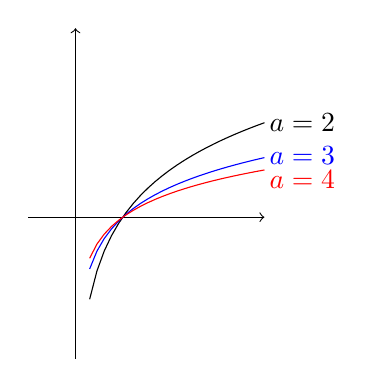
\begin{tikzpicture}[scale=0.6]
            \draw[<->](4,0)--(0,0)--(0,4);
            \draw(0,-3)--(0,0)--(-1,0);
            \draw[black,domain=0.3:4] plot(\x,{log10(\x)/log10(2)}) node at (4.8,2) {$a=2$};
            \draw[blue,domain=0.3:4] plot(\x,{log10(\x)/log10(3)}) node at (4.8,1.3) {$a=3$};
            \draw[red,domain=0.3:4] plot(\x,{log10(\x)/log10(4)}) node at (4.8,0.8) {$a=4$};
        \end{tikzpicture}
        \caption{$a>1$，函数单调增}
    \end{minipage}
    \hfill
    \begin{minipage}[b]{0.45\textwidth}
        \centering
        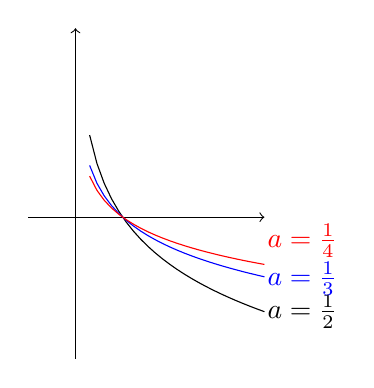
\begin{tikzpicture}[scale=0.6]
            \draw[<->](4,0)--(0,0)--(0,4);
            \draw(0,-3)--(0,0)--(-1,0);
            \draw[black,domain=0.3:4] plot(\x,{-log10(\x)/log10(2)}) node at (4.8,-2) {$a=\frac{1}{2}$};
            \draw[blue,domain=0.3:4] plot(\x,{-log10(\x)/log10(3)}) node at (4.8,-1.3) {$a=\frac{1}{3}$};
            \draw[red,domain=0.3:4] plot(\x,{-log10(\x)/log10(4)}) node at (4.8,-0.5) {$a=\frac{1}{4}$};
        \end{tikzpicture}
        \caption{$a<1$，函数单调减}
    \end{minipage}
    \caption{对数函数 $y=\log_a x$ 的图像}
\end{figure}

\begin{theorem}[对数函数的极限]
    $$
        \begin{aligned}
             & \ln e=1                                    \\
             & \ln 1=0 .                                  \\
             & \lim _{x \rightarrow+\infty} \ln x=+\infty \\
             & \lim _{x \rightarrow 0} \ln x=-\infty .
        \end{aligned}
    $$
\end{theorem}

\begin{center}
    \begin{tabular}{|c|m{5.8cm}|m{5.8cm}|}
        \hline

        \textbf{图像}  &
        % a > 1 的对数函数图像
        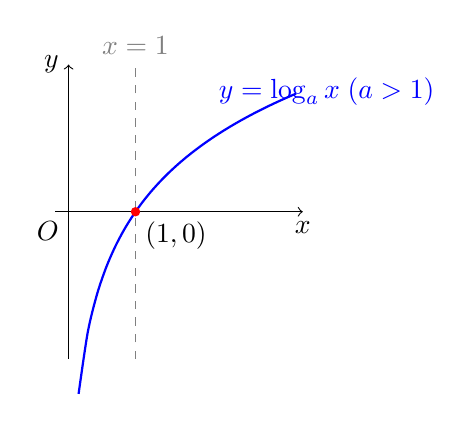
\begin{tikzpicture}[scale=0.85, baseline=(current bounding box.center)]
            % 坐标轴
            \draw[->] (-0.2,0) -- (3.5,0) node[below] {$x$};
            \draw[->] (0,-2.2) -- (0,2.2) node[left] {$y$};
            \node[below left] at (0,0) {$O$};
            % 辅助线 x=1
            \draw[dashed, gray] (1,-2.2) -- (1,2.2) node[above] {$x=1$};
            % 函数曲线
            \draw[domain=0.15:3.4, smooth, variable=\x, blue, thick] plot (\x, {log2(\x)});
            % 标签和点
            \node[blue, right] at (2.1, 1.8) {$y=\log_a x\; (a>1)$};
            \fill[red] (1,0) circle (2pt);
            \node[below right] at (1,0) {$(1,0)$};
        \end{tikzpicture}
                     &
        % 0 < a < 1 的对数函数图像
        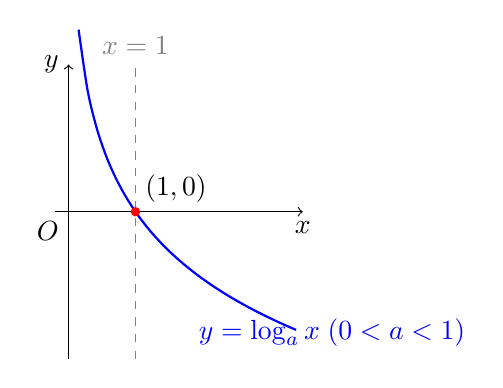
\begin{tikzpicture}[scale=0.85, baseline=(current bounding box.center)]
            % 坐标轴
            \draw[->] (-0.2,0) -- (3.5,0) node[below] {$x$};
            \draw[->] (0,-2.2) -- (0,2.2) node[left] {$y$};
            \node[below left] at (0,0) {$O$};
            % 辅助线 x=1
            \draw[dashed, gray] (1,-2.2) -- (1,2.2) node[above] {$x=1$};
            % 函数曲线
            \draw[domain=0.15:3.4, smooth, variable=\x, blue, thick] plot (\x, {-log2(\x)});
            % 标签和点
            \node[blue, right] at (1.8, -1.8) {$y=\log_a x\; (0<a<1)$};
            \fill[red] (1,0) circle (2pt);
            \node[above right] at (1,0) {$(1,0)$};
        \end{tikzpicture}
        \\
        \hline
        \textbf{定义域} & \multicolumn{2}{c|}{$(0, +\infty)$} \\
        \hline
        \textbf{值域}  & \multicolumn{2}{c|}{$\mathbb{R}$}   \\
        \hline
        \textbf{性质}  &
        \begin{enumerate}
            \item 过定点 $(1, 0)$，即 $x=1$ 时，$y=0$
            \item 在 $(0, +\infty)$ 上是增函数
        \end{enumerate}
                     &
        \begin{enumerate}
            \item 过定点 $(1, 0)$，即 $x=1$ 时，$y=0$
            \item 在 $(0, +\infty)$ 上是减函数
        \end{enumerate}
        \\
        \hline
    \end{tabular}
\end{center}

\subsection{指数函数和对数函数}

不难发现指数函数和对数函数是存在反函数对应关系的。

例如$y=e^x$和$y=\ln x$互为反函数，他们的图像关于直线$y=x$对称。

\subsection{对数函数恒过定点}

\begin{example}
    已知函数 $y=\log _a(x-15)+4(a>0, a \neq 1)$ 过定点 $P$ ，幂函数的图象经过点 $P$ ，则该幂函数的大致图象是（$\quad$）
\end{example}

\begin{figure} [H]
    \centering
    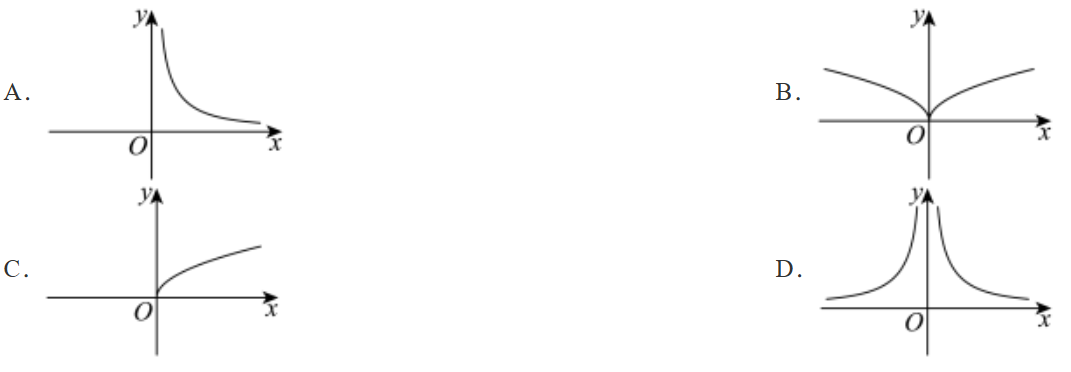
\includegraphics[width=0.7\textwidth]{chapters/函数/images/幂指对函数/img-20250804121655.png}
\end{figure}

\subsection{特殊的奇函数}

\begin{theorem}[特殊的奇函数]
    有时奇函数无法通过 $f(-x)=-f(x)$ 来证明，但可以通过 $f(-x) + f(x) = 0$ 来证明。
\end{theorem}

\begin{example}
    已知函数 $f(x)=\ln \frac{1}{\mathrm{e}^2\left(\sqrt{1+4 x^2}-2 x\right)}$ ，则：
    \begin{itemize}
        \item 函数 $f(x)$ 的单调递增区间为 \underline{\qquad} ；
        \item 若 $f(a+2)+f(5 a+2)+4>0$ ，则实数 $a$ 的取值范围为 \underline{\qquad}.
    \end{itemize}
\end{example}

\v{8em}

\begin{example}
    已知函数 $f(x)=\ln \left(\sqrt{1+x^2}-x\right)+3$ ，并且 $f(m)=2$ ，那么：
    \begin{itemize}
        \item $f(-m)$ 的值为 \underline{\qquad}；
        \item 不等式 $f(x)+f(x-2)<6$ 的解集是 \underline{\qquad}.
    \end{itemize}
\end{example}

\v{8em}

\begin{example}
    已知 $f(x)=\ln \left(\sqrt{x^2+1}+x\right)+\frac{2^x-1}{2^x+1}$
    \begin{itemize}
        \item 若 $f(a)=2$ ，则$f(-a)=$ \underline{\qquad}；
        \item 若 $f\left(\log _{\frac{1}{3}} x^2-1\right) \geq 0$ ，则实数 $x$ 的取值范围是 \underline{\qquad}.
    \end{itemize}
\end{example}

\v{8em}

\subsection{对数函数的单调性}

\begin{example}
    已知函数 $f(x)=\ln \frac{x+1}{1-x}$ ．
    \begin{enumerate}
        \item 判断并证明函数 $f(x)$ 的单调性；

        \item 若 $f(x-3)+f\left(-\frac{1}{2}\right)<0$ ，求实数 $x$ 的取值范围．
    \end{enumerate}
\end{example}

\begin{problemset}
    \item 解方程：$3^x+4^x+5^x = 6^x$
\end{problemset}